% -*- latex -*-
%-----------------------------------------------------------------------
%;  Copyright (C) 2012
%;  Associated Universities, Inc. Washington DC, USA.
%;
%;  This program is free software; you can redistribute it and/or
%;  modify it under the terms of the GNU General Public License as
%;  published by the Free Software Foundation; either version 2 of
%;  the License, or (at your option) any later version.
%;
%;  This program is distributed in the hope that it will be useful,
%;  but WITHOUT ANY WARRANTY; without even the implied warranty of
%;  MERCHANTABILITY or FITNESS FOR A PARTICULAR PURPOSE.  See the
%;  GNU General Public License for more details.
%;
%;  You should have received a copy of the GNU General Public
%;  License along with this program; if not, write to the Free
%;  Software Foundation, Inc., 675 Massachusetts Ave, Cambridge,
%;  MA 02139, USA.
%;
%;  Correspondence concerning AIPS should be addressed as follows:
%;          Internet email: aipsmail@nrao.edu.
%;          Postal address: AIPS Project Office
%;                          National Radio Astronomy Observatory
%;                          520 Edgemont Road
%;                          Charlottesville, VA 22903-2475 USA
%-----------------------------------------------------------------------
%Body of final AIPSletter for 31 December 2011

\documentclass[twoside]{article}
\usepackage{graphics}

\newcommand{\AIPRELEASE}{December 31, 2012}
\newcommand{\AIPVOLUME}{Volume XXXII}
\newcommand{\AIPNUMBER}{Number 2}
\newcommand{\RELEASENAME}{{\tt 31DEC12}}
\newcommand{\OLDNAME}{{\tt 31DEC11}}
\newcommand{\NEWNAME}{{\tt 31DEC13}}

%macros and title page format for the \AIPS\ letter.
\input LET98.MAC

\newcommand{\MYSpace}{-11pt}

\normalstyle

\section{General developments in \AIPS}

\subsection{Reduction of EVLA and ALMA data in \AIPS}

This \Aipsletter\ and those beginning in 2010 documents numerous
improvements to \AIPS\ that enable full calibration of EVLA data and
most imaging operations as well.  The one exception is the wide-band
(bandwidth synthesis) deconvolution algorithm (``MSMFS'') being
developed in \CASA\ by Urvashi Rao Venkata, for which there is no
comparable function in \AIPS\@.  Calibrated $uv$ data may be exported
from \AIPS\ in ``UVFITS'' format for use in that program.  ALMA data
may also be reduced in \AIPS, although the package is not fully
qualified to calibrate data from linearly-polarized feeds.  See
Appendix E of the \AIPS\ Cookbook, available via the \AIPS\ web site,
for details.

\subsection{\Aipsletter\ publication}

We have discontinued paper copies of the \Aipsletter\ other than for
libraries and NRAO staff.  The \Aipsletter\ will be available in
PostScript and pdf forms as always from the web site listed above.  It
will be announced in the NRAO e-News mailing and on the bananas list
server.

\subsection{Current and future releases}

We have formal \AIPS\ releases on an annual basis.  We recommend a
full binary installation method for both the frozen and development
versions for MacIntosh OS/X (PPC and Intel chips), Solaris, and Linux
(32- and 64-bit) systems, but all architectures can do a full
installation from the source files.  If you develop \AIPS\ code
locally {\it or have system managers that forbid the use of\/} {\tt
  rsync}, you will need to do a source-level installation.  The
current release is called \RELEASENAME\ and is now ``frozen.''  If you
took a development copy of this version at some earlier date, you
should use the ``Midnight Job'' (MNJ) to bring it up to date.  You
need to run a MNJ only once in 2013 to convert your copy of
\RELEASENAME\ into the frozen version.  However, when patches to
\RELEASENAME\ are announced, you may apply them with the MNJ\@.  This
\Aipsletter\ is intended to advise you of corrections and improvements
in this release.

We have begun a new version, called \NEWNAME, which is now under
development by the \AIPS\ Group.  You may fetch and install a complete
copy of this version at any time.  Having fetched \NEWNAME, you may
update your installation whenever you want by running the MNJ\@.  This
uses {\tt cvs}, {\tt rsync}, and/or transaction files to copy all
changed text files and then to copy the binary files or to compile the
code selectively based on the code changes and compilations we have
done.  We expect users to take their source-only or binary version of
\NEWNAME\ \AIPS\ over the Internet (via \emph{anonymous} ftp).  Both
versions require you to copy the installation procedure {\tt
  install.pl} via {\tt ftp}; the source-only version also requires you
to ftp the 115-Mbyte {\tt   \NEWNAME.tar.gz} compressed tar file.
Linux sites will almost certainly have {\tt cvs} installed; other
sites may have installed it along with other GNU tools.  Secondary
MNJs will still be possible using {\tt ssh} or {\tt rcp} or NFS as
with previous releases.  We have found that {\tt cvs} works very well,
although it has one quirk. If a site modifies a file locally but in an
\AIPS-standard directory, {\tt cvs} will detect the modification and
attempt to reconcile the local version with the NRAO-supplied version.
This usually produces a file that will not compile or run as intended.
Use a new name for the task or put a copy of the task and its help
file in a private disk area instead.

\AIPS\ is now copyright \copyright\ 1995 through 2012 by Associated
Universities, Inc., NRAO's parent corporation, but may be made freely
available under the terms of the Free Software Foundation's General
Public License (GPL)\@.  This means that User Agreements are no longer
required, that \AIPS\ may be obtained via anonymous ftp without
contacting NRAO, and that the software may be redistributed (and/or
modified), under certain conditions.  The full text of the GPL can be
found in the \texttt{15JUL95} \Aipsletter\ and is included with every
distribution in file {\tt \$AIPS\_ROOT/{\it release-name}/COPYING}\@.


\subsection{Installing a new version}

If compiling locally, new releases must be installed from the tar ball
for that release.  If using the binary installation, a full new
installation must also be done with {\tt rsync}.  The {\tt cvs} system
requires this.  When installing a new \AIPS\ release in a system that
already has a previous release, we recommend that {\tt install.pl} be
used and that the previous release be left in place, at least until
the new installation has been verified.  If you do this, then you will
not have to re-edit the disk, printer, and tape lists and can simply
skip all those pages in the {\tt install.pl} menus.  The old {\tt
  \$HOME/.AIPSRC} file may be left in place, but it will need to be
edited.  The lines giving the {\tt DOWNLOADED} and {\tt UNPACKED}
parameters should be cleared and the {\tt CCOMOPT} line should be
changed to point to the current release rather than the previous one.
If you have made a special version of {\tt do\_daily.{\it host}}, you
should preserve it under a new name and restore it after the install.
If you have an odd set of \AIPS\ versions, the {\tt
  \$AIPS\_ROOT/AIPSPATH.*SH} files may need to be edited after the
install to set the desired versions.

{\tt 31DEC09} contains a change in the format of antenna files.
Previous releases will not understand the antenna coordinates for
arrays that were traditionally left-handed (VLBI primarily).  The
format change occurs automatically when any {\tt 31DEC09} or later
antenna-file specific code reads the file, after which older releases
will have difficulties.  Note that the only version which we patch for
major errors is \RELEASENAME; even \OLDNAME\ is no longer changed.

\section{Preview of coming attractions}

The \NEWNAME\ release already contains a few changes that we decided
were a bit risky or not needed in \RELEASENAME\@.  {\tt SNPLT} was
changed to allow the plotting of multiple parameters from the same
extension table (such as Psum, Pdif, and Psys from the {\tt SY}
table).  {\tt SETJY} was changed to avoid setting {\tt CALCODE} and
the velocity parameters on {\tt OPTYPE}s intended for other purposes.
It will soon have a complete set of spectral parameters as a function
of epoch for the primary calibration sources.  {\tt RFLAG} offers the
option of finding and then using separate amplitude scaling factors
for each IF, baseline, and source.  This will help when the RFI is so
bad that the recommended pre-calibration is not feasible.  {\tt TVFLG}
and {\tt SPFLG} were changed to display the status line in the same
graphics plane as the axis labeling (to enable later displays) and to
offer the option of plotting the data as far to the right as possible,
reducing overlap with the menu.

\vfill\eject

\section{Improvements of interest to users in \RELEASENAME}

We expect to continue publishing the \Aipsletter\ every six months
along with the annual releases.  There are a few new tasks released in
the last six months.  New tasks in the last six months include {\tt
  BSCAN} to find the ``best'' scan on a calibration source to use for
fringe finding and the like, {\tt GCPLT} to plot gain versus elevation
from the input text files used by {\tt INDXR}, {\tt CC2IM} to make
images from Clean Component files, {\tt MODIM} to construct model
image cubes including polarization, spectral index, and rotation
measure, {\tt QUXTR} to extract text files from Q/U cubes for input to
{\tt TARS} (Faraday rotation measure synthesis test task), and {\tt
  TARPL} to plot the output of {\tt TARS}\@.  New verbs include {\tt
  CHARMULT} to intruct the TV display ({\tt XAS}) to use larger
character sizes, {\tt CODECIMAL} to switch coordinates between decimal
and sexagesimal forms, {\tt GETVERS} and {\tt QGETVERS} to return the
maximum version number of a specified extension file type, and
{\tt M2CAT}, {\tt M3CAT}, {\tt M4CAT}, {\tt MOCAT}, {\tt U2CAT},
{\tt U3CAT}, {\tt U4CAT}, and {\tt UOCAT} to do quick catalog listings
of images or $uv$ files for {\tt IN2DISK}, {\tt IN3DISK}, {\tt
  IN4DISK}, and {\tt OUTDISK}, respectively.

In the first six months of \RELEASENAME\ the new tasks were {\tt
  MORIF} to break up a data set into a greater number of spectral
windows, {\tt SNREF} to determine which reference antenna would
minimize the right minus left phase difference, {\tt PRTSY} to print
statistics of the values in SysPower ({\tt SY}) tables from the EVLA,
{\tt FIXAN} to correct errors or change the array center in antenna
tables, {\tt SPCOR} to correct an image cube for spectral index and/or
primary beam, {\tt   FIXRL} to fix data for mislabeled polarizations
in some antennas, and {\tt TARS} to check the Faraday Rotation
Synthesis algorithm (task {\tt FARS}) with simple user input data.
New verbs include {\tt NAMEGET} to fill in the file naming adverbs
completely to aid in writing procedures and {\tt IM2HEAD}, {\tt
  IM3HEAD}, {\tt IM4HEAD}, {\tt IMOHEAD}, {\tt Q2HEADER}, {\tt
  Q3HEADER}, {\tt Q4HEADER}, and {\tt QOHEADER} to display headers
selected by the second, third, and fourth input and the output name
adverbs, respectively.  New {\tt RUN} files include {\tt OOCAL} to
enable full self-calibration with the spectral-index and other options
of the {\tt OOSUB} task and {\tt   LINIMAGE} to build a {\tt FLATN}ed
spectral cube while separating spectral windows to improve performance
in the {\tt IMAGR} portion.

Normally, bugs which are created in an \AIPS\ {\tt TST} version and
then fixed in that same version before its release get little or no
discussion in the \Aipsletter\@.  Since a rather large number of sites
now install the {\tt TST} version of \AIPS\ during its development,
this is somewhat of an oversight.  We urge you to run the ``Midnight
Job'' at least once after \RELEASENAME\ is frozen to bring it up to
date and to fix all bugs of this sort.  We urge active sites to use
the MNJ and, when something odd occurs, to examine {\tt CHANGE.DOC}
using the cgi tool available from the \AIPS\ web page under
documentation.  Please do not hesitate to e-mail {\tt daip@nrao.edu}
with any questions or suspicions that there are problems.

\subsection{UV data}

\begin{description}
\myitem{FRING} was given the {\tt DOAPPLY} adverb to control whether
           single-source data sets would be copied, correcting for the
           calibration parameters found.  The writing of the output
           files now includes automatic generation of an {\tt NX}
           table.  An option to break the input IFs into $N$ groups
           (of equal size) was added, replacing the limit that $N = 1,
           2,$ or 4.  Handling of the case $N=1$ with multi-band
           delays was corrected.  Adverbs {\tt BIF} and {\tt EIF} were
           added but only for the case $N > 0$ and $N \ne\ N_{{\rm
           if}}$.
\myitem{LISTR} was given the option in {\tt DPARM(10)} to control the
           data scaling in {\tt LIST}, {\tt GAIN}, and {\tt MATX}
           modes.
\myitem{Flag} application is now limited to no more than 60000 flags
           applying to a single time in most tasks and 600000 in {\tt
           UVCOP} and {\tt TYAPL}\@.
\myitem{TYAPL} was given the option to apply the post-detection gain
           from the {\tt SY} table rather than the gains determined
           from $P_{{\rm dif}}$.  EVLA 3-bit data benefit from this,
           while the $P_{{\rm dif}}$ values are found to have
           non-linear scaling issues.
\myitem{UVCOP} copies tables for a time range beginning a little
           before that used for the $uv$ data and ending a little
           after so that enough table values will be available for any
           interpolation.  User control over the size of ``little''
           was added.  The copying of {\tt PD} tables (spectral
           polarization calibration) was corrected.
\myitem{RFLAG} was changed to handle {\tt FG} table versions more
           carefully to achieve the apparent user-requested pattern.
           Since this task uses the flag table to read the data
           multiple times, but also can write it at the same time,
           great care is required.
\myitem{CLCOR} was changed to re-compute the apparent coordinates
           before using them in source and antenna position
           corrections.  {\tt FITLD} was changed to re-compute the
           apparent coordinates in all cases, not just those in which
           they were very obviously wrong.
\myitem{Ka-band} models for the primary flux calibration sources were
           released.
\myitem{EVAUV} was changed to plot the real versus imaginary values of
           the data-model and data/model-1 files as logarithmic
           contours in 2-dimensional images.  Adverbs to control these
           plots (size of images, range of values, smoothing) were
           added.  The option of saving the data-model and data/model
           $uv$ data sets was also added.
\myitem{UVFIX} was made fault tolerant when it fails to find a
           particular source, time, and antenna in the {\tt CL} table
           or {\tt FO} table.  It used to turn off all time-dependent
           frequency shifts in case of error, but now reports the
           error and keeps trying.
\myitem{ATLOD} was corrected to handle files larger than 2 Giga-bytes.
\myitem{CLCOP} was given an {\tt AVER} option to average values from a
           list of IFs and then replace the values of another list of
           IFs with the average.  This should help deal with IFs
           adversely affected by RFI, line emission, and the like.
\myitem{SETJY} was corrected for errors in {\tt OPTYPE 'VCAL'} in
           computing LSR and radio-convention velocities\@.  The
           transfer of velocity at one pixel to that at the reference
           pixel in the optical convention was replaced by the more
           accurate, fully non-linear formula.  Perley-Butler fluxes
           for 2013 were added for 3C286 and 3C295 (only) and the
           reporting of the ``previous'' values was improved.
\myitem{TVFLG} and {\tt SPFLG} had addressing problems after the {\tt
           MAXCHA} increase which could cause the master grid to be
           damaged on {\tt CLIP INTERACTIVE}, while {\tt LIST FLAGS}
           needed modernizing to report them correctly and {\tt NEXT
             IF/ST} assumed 2 Stokes without checking which made for
           addressing problems.
\myitem{BSCAN} is a new task which checks the data in each scan of a
           user-specified calibrator source to see if any have all
           antennas and, if so, which has the most data.  It returns
           time ranges of the recommended scans.  This should be most
           useful in pipelines searching for fringe finder scans and
           the like.
\myitem{GAINS} for the EVLA antennas as functions of elevation are
           given in a text file determined by Perley and Butler.  The
           file was corrected and currently only has one set of values
           for each band although it retains the ability to be more
           finely divided in frequency.
\myitem{Baseline} dependent calibration may be determined with {\tt
           BLCAL} and then applied through adverb {\tt BLVER}\@.  The
           calibration routines failed to initialize its use properly
           which caused confusion in tasks like {\tt IMAGR} that read
           different $uv$ files through the calibration routines.
\myitem{Edit} class methods used in {\tt EDITA}, {\tt EDITR}, {\tt
           SNEDT} and others were changed the make the {\tt SWITCH ALL
           IF} operation have 3 possibilities: 1 IF, a range of IFs,
           and all IFs.  The second one is new and appropriate for
           EVLA data in some cases.
\myitem{KEYIN} is a routine used to parse free-format inputs for
           tasks including {\tt PCLOD}, {\tt SETAN}, {\tt USUBA},
           {\tt M3TAR}, {\tt DTSIM}, {\tt ANCAL}, {\tt FETCH}, {\tt
             ANTAB}, {\tt VLBIN}, {\tt UVFLG}, and {\tt MK3IN}\@.
           Its handling of character strings owes more to Fortran 2
           than 77 and required a variety of fixes to handle strings
           of varying lengths.
\end{description}

\subsection{Imaging}

Compared to some years, {\tt IMAGR} has received only modest
attention.  It was changed to compute the actual average frequency
found in the data used to make a bandwidth-synthesis image and to put
that frequency in the header.  Editing can cause this to be somewhat
different from the nominal frequency.  The findings of this
computation are reported to the user.  Errors in frequency-dependent
imaging were found: the value of {\tt FQTOL} could get lost causing
the task to do way too much work and too low a value for the number of
channels could get used, causing the model to be damaged.  When {\tt
  IMAGR} was told to include all subarrays but also given other adverb
values (such as time range) that caused there to be no data in one or
more of the subarrays, the task would die.  It was corrected to handle
the ``no data'' return with grace, dying only if all subarrays lack
data.  Subtle errors affecting multi-facet imaging with {\tt ONEBEAM}
true and cases in which baseline-dependent calibration is to be
applied were also corrected.


\subsection{Faraday rotation analysis}

The subject of Faraday rotation measure synthesis is receiving a great
deal of attention these days.  \AIPS\ task {\tt FARS} performs this
analysis and was corrected to subtract the contribution of the last
Clean component from the residuals before they are used for output or
for restoration of the components.  The output file naming adverbs
were simplified and the header coordinates corrected to drop the
incorrect {\tt STOKES} axis.  Task {\tt AFARS} examines the image
cubes from {\tt FARS} to extract images of the rotation measure at the
peak amplitude and the amplitude and phase or real and imaginary at
that peak (along the RM axis).  The methods of determining that
maximum were changed, with the new default being an exact cubic fit,
and with obviously wrong answers trapped and corrected.  {\tt AFARS}
now writes out all 3 images with a simplified control of the output
names and with corrected header coordinates.

To study the methods used in {\tt FARS}, another task {\tt TARS} was
written.  It computes a single rotation measure spectrum, taking its
data from an input text file which can include model components and a
spectrum of Q and U values and writing an output text file.  It had
the same error as {\tt FARS} in handling the last Clean component.
{\tt TARS} was changed to use the sum of the Q/U spectrum and any
model.  Previously, it ignored the Q/U values if there was a model and
used the spectrum only for its list of frequencies.  An experimental
method of doing a complex Clean was added.  This pattern match scheme
is rather slow and so will not be added to {\tt FARS} unless it is
found to be worth the wait.  the width of the real part of the RM
transfer function (dirty beam really) is now used as the default
restoring beam width.  {\tt TARS} may now write repeatedly to the same
output text file, allowing comparison of RM spectra made with
different input parameters.

To assist in these studies, three new tasks were also written.  {\tt
  MODIM} will construct model I, Q, and U cubes.  Each model component
has I, Q, U fluxes at 1 GHz plus a spectral index and rotation measure
as well as the usual position, width, and type parameters.  Up to 9999
components may be read from a text file and, optionally, added to
pre-existing images.  New task {\tt QUXTR} reads Q and U cubes to
extract a spectrum in the form expected by {\tt TARS}\@.  Finally, new
task {\tt TARPL} plots the RM spectrum from one or more {\tt TARS}
output spectra contained in a single text file.

\subsection{Other analysis}

\begin{description}
\myitem{SLICE} was given the option to avoid interpolation when the
           slice is directly along the $X$ or $Y$ axis.  It already
           did that along the $Z$ axis.  It now allows non-integer end
           points when interpolating.  All slice plots and {\tt SLFIT}
           now detect the old format slice files and handle them
           correctly.  The format was changed quite some time ago
           without properly insuring backward compatibility.
\myitem{CODECIMAL} \hspace{2em} is a new verb to switch between
           decimal coordinate ({\tt X}, {\tt Y}) and sexagesimal
           coordinate ({\tt COORDINA}) representations.
\myitem{IMVAL} was changed to let the user choose between returning
           the value at the nearest integer pixel and doing a cubic
           fit to determine the value.
\myitem{MAXFIT} was changed to return the shift necessary to move the
           peak found to the nearest integer pixel.
\myitem{CC2IM} is a new task to convert point and Gaussian components
           in Clean Component extension files into images without any
           convolution.  Some software expects model images rather
           than {\tt CC} files.
\myitem{FITLD} and {\tt IMLOD} now trap the modern coordinate
           description used for East-West interferometers and change
           it into the description recognized by \AIPS\ ({\tt
             -NCP})\@.
\end{description}

\subsection{Display}

\begin{description}
\myitem{SNPLT} was given the option to color the plot based on source
           number.  This is very helpful when examining calibration
           tables.
\myitem{IMEAN} now uses {\tt BLC}, {\tt TRC}, and {\tt DOINVERS} when
           it does the initial robust estimate of the rms prior to the
           fitting.  {\tt DOMODEL} was added to control the plotting
           of the fit Gaussian.  The {\tt TRIANGLE} adverb was added
           to output the flux level exceeded by only $i$ percent of
           the pixels.  This may be used in scripts to select
           intensity ranges, contour levels, and the like.
\myitem{POSSM} was changed to avoid plot labels below panels that are
           not the bottom of a column of panels.  Overlaps were
           occurring in {\tt LWPLA} outputs.  Labeling of IF numbers
           and polarization was improved.  The flux scaling (milli,
           kilo, {\it et al.} will now be fixed on each plot page,
           being set by the first panel.  Previously, when panels were
           separately scaled, the prefix portion was ambiguous.
\myitem{GREYS} was corrected to handle 3-color images correctly and
           was given additional options controlling the transfer
           function type and intensity ranges separately in each
           color.  {\tt KNTR} and {\tt PCNTR} were also corrected to
           implement {\tt DOCOLOR} correctly.
\myitem{TVHUI} was changed to allow transfer functions in the hue
           image and to allow the output of an image of a
           two-dimensional, hue-intensity step wedge.
\myitem{LWPLA} was changed to guess the size of characters in a string
           (some are narrow) and adjust the string positioning
           accordingly.  Plot tasks will now use upper and lower case
           lettering where appropriate.  Plots now can have ticks
           separated by as little as 1 micro unit (previously 10 micro
           units was the lower limit).
\myitem{PRTAB} was changed to use F format by default for printing
           real and double precision values.  It tries to represent
           both the smallest and largest values present.
\myitem{GCPLT} is a new task to plot the gain curve text files used by
           {\tt INDXR} and {\tt BDF2AIPS}\@.
\myitem{TAPLT} was given more adverbs to limit which rows are selected
           for inclusion in the plot.
\myitem{EXTLIST} was brought up to date systematically for all plot
           tasks already supported and support for {\tt CCNTR}, {\tt
           SERCH}, {\tt EVAUV}, {\tt DELZN}, {\tt ELINT}, {\tt FGPLT},
           {\tt GAL}, {\tt SNIFS}, {\tt SOUSP}, and {\tt WETHR} was
           added.  These tasks were modified to insure that defaults
           were filled in before the plot files are created.  Verb
           {\tt PLGET} was also updated to support these tasks.
\myitem{CHARMULT} \hspace{2em} is a new verb to instruct the {\tt XAS}
           TV display to use the standard character font scaled by a
           specified integer.  Very large TV displays will choose the
           default scaling but may need user direction.
\end{description}

\subsection{General and system matters}

\begin{description}
\myitem{MAXCHA} is the maximum number of spectral channels which
           \AIPS\ can handle.  It was increased from 65536 to 132096
           (a factor of 2 plus 1024).  An overflow in the calibration
           application at 65536 was corrected.
\myitem{TAB} characters in input text files are invisible to users and
           catastrophic to incautious software.  All software was
           changed to check input text for TABs and change them to an
           equal number of blanks.
\myitem{CookBook} was updated generally including Appendix E specifically
           addressed to EVLA users.  The control files that enable TAB
           completion, {\tt ABOUT}, and {\tt APROPOS} were also updated.
\myitem{U2CAT,} {\tt U3CAT}, {\tt U4CAT}, and {\tt UOCAT} are new
           verbs like {\tt UCAT} except that the disk examined is
           controlled by the {\tt IN2DISK}, {\tt IN3DISK}, {\tt
           IN4DISK}, and {\tt OUTDISK} adverbs, respectively.
\myitem{M2CAT,} {\tt M3CAT}, {\tt M4CAT}, and {\tt MOCAT} are new
           verbs like {\tt MCAT} except that the disk examined is
           controlled by the {\tt IN2DISK}, {\tt IN3DISK}, {\tt
           IN4DISK}, and {\tt OUTDISK} adverbs, respectively.
\myitem{GETVERS} is a new verb to return the maximum version number of
           the extension file type specified with messages; {\tt
           QGETVERS} does the same, but quietly.  The output is stored
           in the {\tt MAXVERS} adverb.
\end{description}
\vfill\eject

\section{Patch Distribution for \OLDNAME}

Because of the extensive use of binary installations, we now patch the
master copy of the most recently frozen version.  Older versions are
not corrected even for egregious errors.  Thus, \OLDNAME\ was patched
during 2012 and \RELEASENAME\ will be patched as needed during 2013.
Your copy of them may be corrected simply by running a Midnight Job.
Information about patches and the code may be found using links from
the main \AIPS\ web page or by  {\it anonymous} \ftp\ to the NRAO
server {\tt ftp.aoc.nrao.edu}.  Documentation about patches to a
release is placed on this site at {\tt pub/software/aips/}{\it
  release-name} and the code is placed in suitable sub-directories
below this.  Patches to older releases are kept here as well, but they
will require local compilation.

The \OLDNAME\ release is no longer available for installation and will
no longer receive patches even for egregious errors.  It had a number
of important patches during 2012.  They are
\begin{enumerate}
  \item\ Imaging code had problems with large gridded modeling.
      {\it 2012-01-16}
  \item\ {\tt UVFIT} had many areas dimensioned for the old limit of 4
      components, rather than the new limit of 20. {\it 2012-01-16}
  \item\ {\tt FARS} did not shift residuals back to the original
      $\lambda^2$ correctly and did not add residuals into
      amplitude/phase outputs correctly. {\it 2012-01-16}
  \item\ {\tt AFARS} did not handle {\tt BLC} correctly, producing
      wrong rotation measure images.  It also stated incorrect
      information in the history. {\it 2012-01-16}
  \item\ {\tt SQASH} had an error in history writing that led to
      aborts.  {\it 2012-01-16}
  \item\ {\tt FITAB} omitted an essential keyword for compressed UV
      data.  {\it 2012-01-16}
  \item\ {\tt CLCOR} ignored the fact that the GMRT uses an opposite
      phase convention. {\it 2012-01-16}
  \item\ {\tt VLANT} did not correct EVLA data properly. {\it
      2012-03-01}
  \item\ {\tt SCMAP} and {\tt SCIMG} did not apply the flag table to
      the data entering the self-cal step {\it 2012-03-07}
  \item\ Mac OS/X version Mountain Lion changed {\tt ps} to issue an
      error message when there is a library path; procedures needed
      defenses against this.  {\it 2012-11-19}
\end{enumerate}

\vfill\eject

\section{\AIPS\ Distribution}

From the NRAO system logs, we count apparent MNJ accesses, downloads
of the tar balls, and {\tt rsync} accesses by unique IP address.
Since DSL and some university and other connections may be assigned
different IP addresses at different times, this will be a bit of an
over-estimate of actual sites.  However, a single IP address is often
used to provide \AIPS\ to a number of computers, so these numbers are
at the same time an under-estimate of the number of computers running
current versions of \AIPS\@.  In 2012, a total of 284 different IP
addresses downloaded the frozen form of \OLDNAME\ and 940 IP
addresses downloaded \RELEASENAME\ in tarball or binary form.  Fully
1309 IP addresses accessed the NRAO cvs master.  Each of these has at
least installed some version of \AIPS\ and 422 appear to have run the
MNJ at least occasionally.  The total number of unique IP addresses in
these three lists was 1698.  The table below shows these numbers as a
function of year since we began recording them.  The attached figure
shows the cumulative number of unique sites, cvs access sites, and
tar-ball/binary download sites known to us as a function of week in
2012.  The numbers for 2011 are also plotted and show a drop in the
shipping of {\tt TST}\@.  The cvs access numbers have dropped in a way
that suggests some change in the manner of counting in addition to the
decrease in the numbers for the {\tt TST} version.

\vfill
\begin{center}
\begin{tabular}{|rrrrrrrrr|}
\hline
%year & {\tt TST} name & {\tt NEW} name & \hspace{1em}{\tt TST} &
% \hspace{1em}{\tt NEW} & {\tt TST binary} & {\tt NEW} binary &
% \hspace{1em}{\tt cvs} & Total unique \\
 & & & & & {\tt TST} & {\tt NEW} & & Total \\
\noalign{\vspace{-1mm}}
year & {\tt TST} name & {\tt NEW} name & \hspace{1em}{\tt TST} &
 \hspace{1em}{\tt NEW} & binary & binary &
 \hspace{1em}{\tt cvs} & unique \\
\hline
2004 & {\tt 31DEC04} & {\tt 31DEC03} &  808 & 196 &      &     &  797
 & 1276 \\
2005 & {\tt 31DEC05} & {\tt 31DEC04} &  832 & 246 &  299 &  48 &  982
 & 1460 \\
2006 & {\tt 31DEC06} & {\tt 31DEC05} &  806 & 191 &  402 &  94 & 1050
 & 1398 \\
2007 & {\tt 31DEC07} & {\tt 31DEC06} &  965 & 277 &  669 & 161 & 1385
 & 1811 \\
2008 & {\tt 31DEC08} & {\tt 31DEC07} & 1058 & 246 &  986 & 303 & 1667
 & 2107 \\
2009 & {\tt 31DEC09} & {\tt 31DEC08} & 1228 & 307 & 1082 & 478 & 1855
 & 2399 \\
2010 & {\tt 31DEC10} & {\tt 31DEC09} & 1228 & 307 & 1203 & 477 & 1914
 & 2416 \\
2011 & {\tt 31DEC11} & {\tt 31DEC10} & 1105 & 270 & 1064 & 424 & 1747
 & 2228 \\
2012 & {\tt 31DEC12} & {\tt 31DEC11} &  940 & 284 & 1028 & 396 & 1309
 & 1698 \\
\hline
\end{tabular}
\end{center}
\vfill
\centerline{\resizebox{!}{4.6in}{\includegraphics{FIG/PLOTIT12b.PS}}}

\eject
\section{Recent \AIPS\ and related Memoranda}

All \AIPS\ Memoranda are available from the \AIPS\ home page.  \AIPS\
Memo 117 describing \AIPS' usage of the FITS format was modified
slightly on several occasions in 2012.  In addition, there are two new
EVLA memorandum from the \AIPS\ group in the last six months.  Obtain
them via\\
\centerline{ {\tt http://www.aoc.nrao.edu/evla/memolist.shtml}}
\vspace{0.1cm}

\begin{tabular}{lp{5.8in}}
{\bf 162} & {\bf Comparison of E and D configuration sensitivity when
      D configuration is tapered}\\
   &  L. Kogan \&\ F. Owen, NRAO\\
   &  July 6, 2012\\
   &  The latest design of the new most compact E-configuration of VLA
has been finished.  So the array dimensions are approximately 3 times
less than the existed most compact VLA configuration: D\@.  Therefore
the sensitivity of E-configuration to the brightness temperature of an
expanded source might be expected to be 9 times better in comparison
with D configuration.  However using tapering with D-configuration
data can diminish this advantage.  In this memo, we estimate the
actual possible advantage of E configuration when tapering is used
with the D configuration data.
\end{tabular}

\vspace{0.1cm}

\begin{tabular}{lp{5.8in}}
{\bf 164} & {\bf Some comments on the W-projection algorithm}\\
   &  Leonid Kogan, NRAO (ret.)\\
   &  October 8 2012\\
   &  The algorithm W-projection implemented in CASA has been
successfully tested using some data.  But still the restrictions of
this algorithm are not clear.  In this memo we point out to the
possible problems at the case of poor UV coverage for some W layers.
We have evaluated analytically the convolution function which is used
at the W-projection algorithm to project (recalculate) the measured
visibilities (corrupted by the W term) to the visibilities
corresponded to the ideal observations (W=0).  The found analytical
equation for the convolution function allows to find a simple
expression for its width for arbitrary field of view and W\@.  The
width is much wider in some cases than the upper limit (70x70 pixels)
cited and therefore the computation time may not be as small as cited.
We suggest multiplication by $\exp(j\pi W l^2)$ at the image plane
(instead of the convolution at the UV plane).  Such a way to correct
the W-term may give the gain in the computation time.
\end{tabular}

\section{Personal note}

Leonia Kogan has retired from NRAO and the \AIPS\ group although he
still pays attention to our progress and will help us if needed with
programs for which he was responsible; note the EVLA Memo cited above.
Leonia worked for NRAO for nearly 20 years, most of that assisting the
\AIPS\ project.  His first {\tt CHANGE.DOC} entry was May 21, 1993.
He is a mathematician by training and temperament and solved many of
our most difficult, mathematically-based issues.  Most recently he
worked on {\tt FARS}, implementing NRAO's first Faraday Rotation
Synthesis algorithm.  But he is also well known for {\tt UVFIX} which
computes $u,v,w$ from antenna locations and time with much trusted
accuracy and for several correction functions in {\tt CLCOR}, most
notably that for the position of the Earth's pole.  He is widely known
for his work on array configurations, represented in \AIPS\ by tasks
{\tt CONFI} (array optimization) and {\tt UVCON} (array simulation)\@.
VLBI data calibration received a lot of his attention through tasks
such as {\tt FRMAP}, {\tt PCCOR}, {\tt PCLOD}, {\tt ACCOR}, {\tt
  COHER}, {\tt DELZN}, and {\tt ATMCA} as well as work on handling
orbiting antenn\ae.  He developed {\tt UVRFI} to excise RFI from EVLA
data and did substantial work on tasks {\tt VPLOT}, {\tt SPLAT}, {\tt
  FGPLT}, {\tt ELINT}, and {\tt RMSD}\@.  Leonia's name appears on
very many entries in {\tt CHANGE.DOC} encompassing a much wider range
of matters than the list given above would suggest and reflecting his
ready willingness to help wherever he was needed.  Leonia will be
missed and we wish him the very best in his future endeavors.
\vfill\eject



% Order form and mailer page
%\cleardoublepage
\pagestyle{empty}
%\vfill
%\centerline{\resizebox{!}{23.3cm}{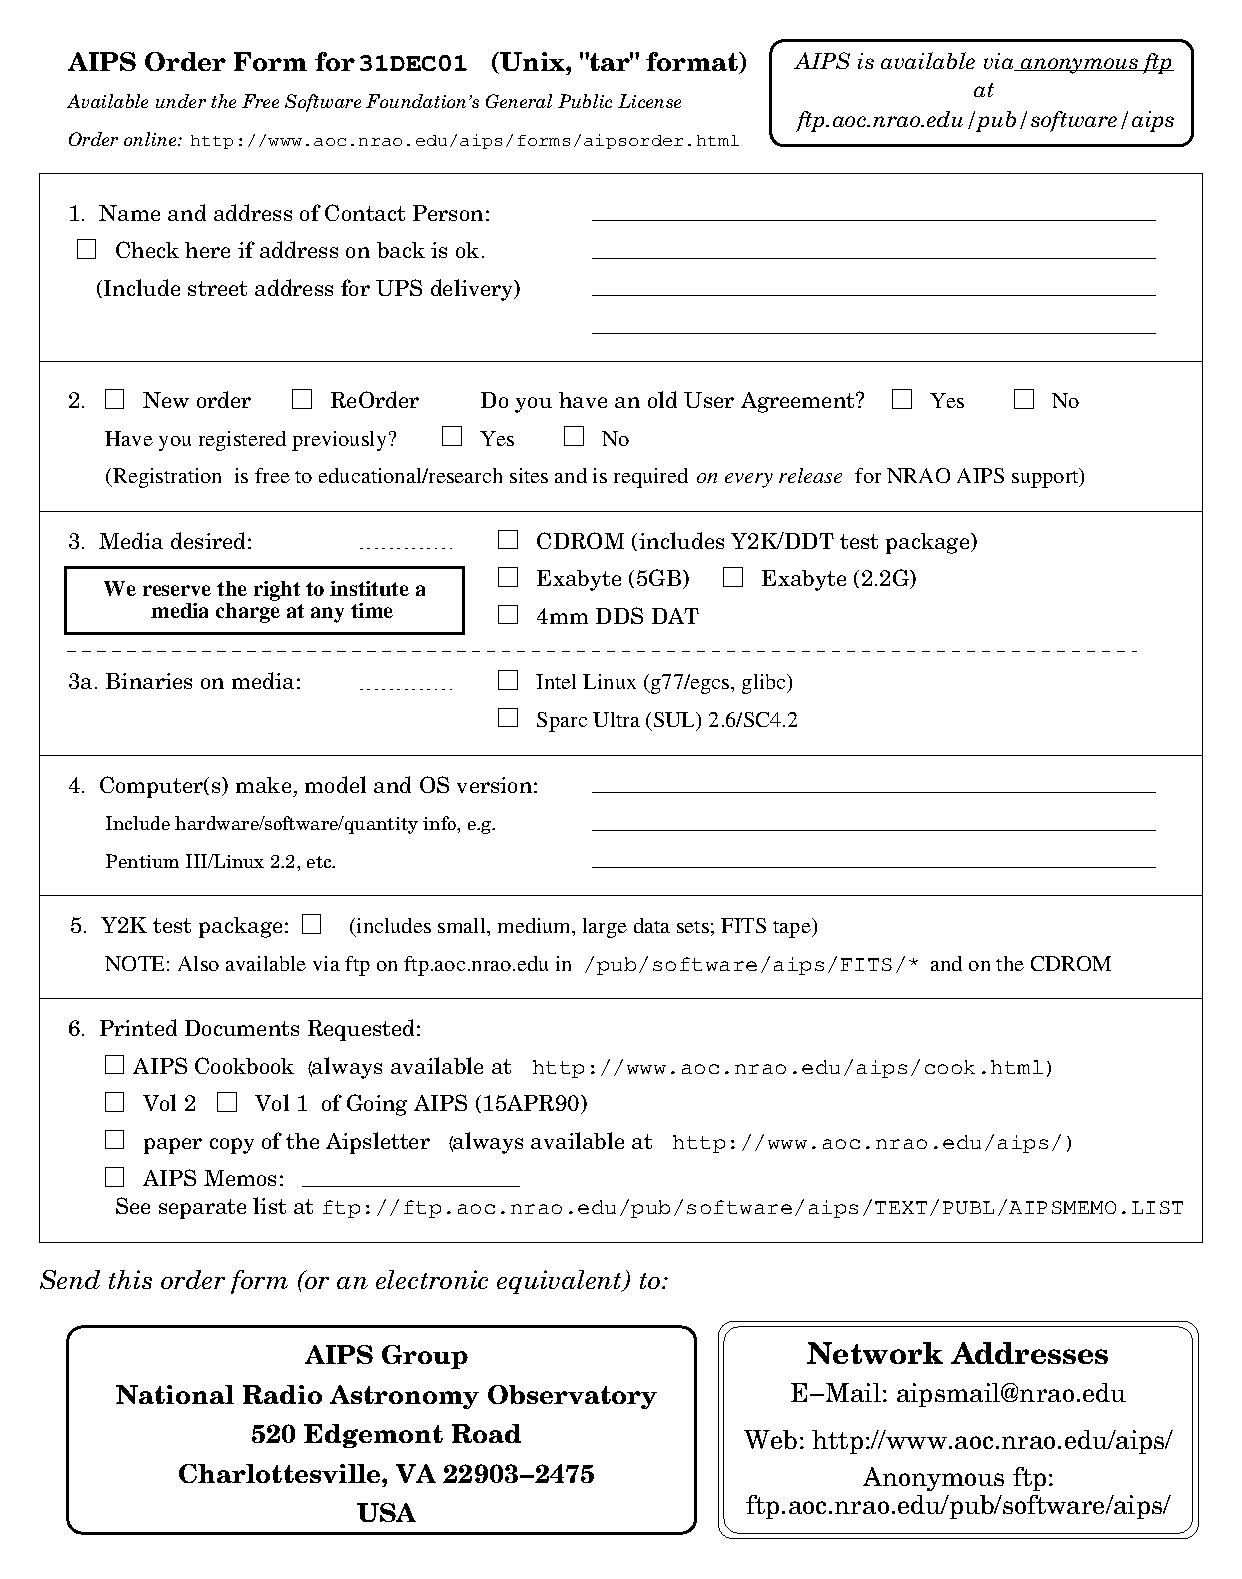
\includegraphics{FIG/AIPSORDER.PS}}}
%\vfill\eject
\vbox to 4.4in{
\vspace{12pt}
%\centerline{\rotatebox{-90}{\resizebox{!}{3.5in}{%
%\includegraphics{FIG/Mandrill.color.plt}}}}
\centerline{\resizebox{!}{3.5in}{\includegraphics{FIG/Mandrill.eps}}}
\vspace{12pt}
\centerline{{\huge \tt \AIPRELEASE}}
\vspace{12pt}
\vfill}
\phantom{...}
\centerline{\resizebox{!}{!}{\includegraphics{FIG/AIPSLETS.PS}}}

\end{document}
